\documentclass[12pt, letterpaper]{article}

% Import Packages ===================================
\usepackage{amsmath} % for for typesetting formulae and equations
\usepackage{amsthm} % for theorem enviornment (load AFTER amsmath)
\usepackage{amssymb} % for (more) mathematical symbols

\usepackage{esint} % more integration symbols

\usepackage{graphicx} % for figures
\usepackage{floatrow}  % for formatting figures and tables
\usepackage{float} % for formatting figures and tables
\usepackage{listings} % to highlight code
\usepackage{hyperref}
\usepackage{url}
\usepackage[a4paper, hmargin=1in, vmargin=1.5in]{geometry}
\usepackage[parfill]{parskip}
\usepackage{ragged2e}
\usepackage{xcolor}

% Listing Environment Setup ===============================
\lstset{
    numbers=left,       % Specify numbering and position
    language=[LaTeX]TeX,% Specify default language
    breaklines=true,    % Breaklines automatically only at whitespaces
    keywordstyle=\color{blue}\bfseries,
    numberstyle=\tiny\color{gray},
    commentstyle=\color{green!30!black},
    stringstyle=\color{violet}
    frameround=fttt
}

% New Environment =========================================
\newcounter{claim} % To create a new counter for numbering the environments (like theorem)
%If you want the counter to reset after every section, add a [section] argument after \newcolor{claim}
%\newcounter{claim}[section]
%\newenvironment{nameofenvironment}[no. of arguments]
%{<code at the beginning>}
%{<ending code>}

\newenvironment{claim}[2][black] % The [black] makes the first argument optional with a default value of black
{ % This cell executes when the \begin{env.} is used
    \color{#1!50!black}
    \refstepcounter{claim} %increments the value of counter by 1

    \begin{center}
        \textbf{\large{Claim \theclaim}} \\ % prints value of counter
        \textbf{#2}
    \end{center}
}
{ % This cell executes when the \end{env.} is used
    \vspace{1.5em} 
}

% Theorem Environment Setup ===============================
\newtheorem{theorem}{Theorem}
\newtheorem{lemma}{Lemma}
\newtheorem{corollary}[theorem]{Corollary}
\newtheorem{proposition}{Proposition}[section]

\theoremstyle{remark}
\newtheorem*{remark}{Remark}

% Title =======================================
\title{Mathematical Report Typesetting}
\author{Prakhar Mittal}


\begin{document}

\maketitle
\tableofcontents
\clearpage

\section{Equations and Formulae}
    \subsection{Math Mode}
    To type maths in \LaTeX{}, one needs to switch to math mode, a special mode in \LaTeX.
    There are 2 tpes of modes: 

    \begin{description}
        \item[Inline Math] The typesetted math sits in the same line as the running text
        and is not typesetted in a math environment, generally used for simple statements
        such as $a=b$ to be embedded inside a line.
        \item[Math enviornment] The mypesetted math sits in its own space,
        generally used for large or important equations or a number of equations.
        
        Generally we don't write text in math enviornment as it would be rendered \textit{likethis}
        without any spacing
    \end{description}

    \subsection{Inline Math}
    For typesetting mathematical expressions in the midst of your text,
    place the expression between two \$ signs. For example :

    If a function $f$ is continuous, then for every $\varepsilon > 0$ there 
    exists a $\delta$ such that $||\mathbf{x}-\mathbf{x_0}|| < \delta$ implies
    $||f(\mathbf{x})-f(\mathbf{x_0})|| < \varepsilon$.\footnotemark
    \footnotetext{$\backslash$varepsilon $\rightarrow \varepsilon$ whereas $\backslash$epsilon $\rightarrow \epsilon$}

    Other ways to typeset inline math is to wrap the expression in:
    \begin{itemize}
        \item \verb!\![  `expression here without the quotes' \verb!\!]
        \item \$\$ `expression here without the quotes' \$\$
    \end{itemize}  
    For small greek letters like $\theta$ we use \verb!\!\textbf{theta}. To capitalize it ($\Theta$) use \verb!\!\textbf{Theta}. \\
    To bold in math we use \verb!\!\textbf{mathbf}. However, this does not work for greek symbols.
    For greek symbols, we use \verb!\!\textbf{boldsymbol}. For example: $\boldsymbol{\omega}$ 

    For using subscripts/superscripts, we use underscore/carat sign before the text in subscript/superscript. If the text does not 
    include any spaces, we can directly use them, eg. $x_0^1$, however, if the text does include spaces, then we have to wrap it in curly braces, eg. 
    $p^{\alpha + \beta}_{ij}$.

    Now consider \$t \verb!\!in \verb!\!mathbb\{R\}\$, this will typeset as
    
    \begin{center}
        $t \in \mathbb{R}$
    \end{center}
    
    See how many other math stuff can be easily typesetted?

    In some cases, we wish to use symbols that otherwise hold a meaning in syntax handling such as
    \$ or \{\}. To escape their special meaning and typeset them as it is, we use backslah followed by the symbols
    (in most cases), like \verb!\!\$.
    
    Tilde creates a space between symbols in inline math mode. For eg.
    
    \begin{center}
        $S :=\{x|~x\equiv 1 \pmod{9}\}$. $T :=\{x|~x \equiv 1\pmod{3}\}$. $S \subset T$ .
    \end{center} (Notice the distance between vertical line and x)

    There are several symbols which can be typesetted using \LaTeX{} (including this one). A comprehensive
    list can be found \href{https://oeis.org/wiki/List_of_LaTeX_mathematical_symbols}{here}.

    Some other math expressions which are commonly used are : 
    \begin{description}
        \item[Combinations] $\binom{n}{k}$ also written as $\frac{n!}{(n-k)!}$
        \item[Continued Product] $n!=\prod_{i=1}^{n} i $ 
        \item[Integration] An extension of factorial function is the Gamma function. For positive integers $n$,
            \begin{center}
                $(n-1)! = \Gamma(n)=\int_{0}^{\infty}x^{n-1}e^{-x}dx$ 
            \end{center}
        \item[Continued Sum] It follows from the Binomial Theorem that $\sum_{k=1}^{n}\binom{n}{k}=2^n$.
        \item[Root] The Binomial Theorem is incredibly powerful and can be used to approximate $\sqrt{1+x},$ 
        or even $\sqrt[71]{1+x}$.
    \end{description}

    Sometimes we want regular text while writing in mah ode, for that we use \verb!\!\textbf{text}.
    For eg. 
    \begin{center}
        $\text{P} \subseteq \text{NP}$. However, we know that testing the positivity of the term
        $\text{residue}(n)$ is decidable in $\text{coNP}^{\text{RP}}$
    \end{center}

    \subsection{The Equation Environment}
    Equations are often pivotal to a report, and they need to stand out. This is where
    the equation environment comes into play. Here's an example: 
    
    \begin{center}
        The Ideal Gas Law states that : 
        \begin{equation}
            pV=nRT
            \label{gaslaw}
        \end{equation}
    \end{center}

    Notice the label (in the source code :P). This helps to refer the equation in later sections.
    Hence, it is a good practice to label the equations.

    Sometmes when you are absolutely sure that an equation would not come into use later (like an intermediate step of a derivation),
    then you would like to do away with the side numbering. This can be done in two ways, 1. using modified equation environment (equation*),
    or by using \verb!\!\textbf{nonumber}. \\ Eg:

    \begin{center}
        Vanderwall Proposed the real gas equation as a more accurate model.
        \begin{equation*}
            \left(p+\frac{an^2}{V^2}\right)(V-nb)=nRT \footnotemark 
        \end{equation*} 
        If you introduce a variable compressibility factor $Z$, this can be ultimately
        expressed as 
        \begin{equation}
            pV=ZnRT \nonumber
        \end{equation}
    \end{center}
\footnotetext{$\backslash$left( $\backslash$right) ensure that the brackets are appropriately sized}

    Many a times, it is required to write several equations one after the other.
    In such cases, it looks nice of they are properly aligned. It is strongly recommended to use the align environment for this,
    which is a part of the amsmath package. \href{https://tex.stackexchange.com/questions/196/eqnarray-vs-align}{Do not use eqnarray, which is simply base \LaTeX.}

    Use \& right before the symbol you want alignment about. Use double backslash ($\backslash \backslash$) for changing line.
    Example: 
    \begin{align*}
        \boldsymbol{\nabla} \cdot \mathbf{E} &= \frac{\rho}{\varepsilon_0} \\
        \boldsymbol{\nabla} \cdot \mathbf{B} &= 0 \\
        \boldsymbol{\nabla} \times \mathbf{E} &= -\frac{\partial \mathbf{B}}{\partial t} \\
        \boldsymbol{\nabla} \times \mathbf{B} &= \mu_0\mathbf{j} + \frac{1}{c^2}\frac{\partial \mathbf{B}}{\partial t} \\
    \end{align*}
    See how the 4 equations are neatly aligned such that all the `=' sign lie on the same line.

    \subsection{Matrices}
    Typesetting matrices is straightforward, very similar to tables. Here's an example:

    The companion matrix $M$ is given as: \\
    $$\begin{bmatrix}
        0 & 1 & 0 & \dots & 0 \\
        0 & 0 & 1 & \dots & 0 \\
        \vdots & \vdots & \vdots & \ddots & \vdots \\
        0 & 0 & 0 & \dots & 1 \\
        a_0 & a_1 & a_2 & \dots & a_{\kappa-1}
    \end{bmatrix}$$
    $M$ is invertible \textbf{iff} $a_0 \neq 0$.

    There are various \href{https://www.overleaf.com/learn/latex/Matrices}{styles of matrices} that the amsmath package allows you to typeset.

\clearpage

    \subsection{Macros: Custom Commands}
    Many a times we need a certain typing style used again and again. If it requires multiple commands, then this work
    becomes quite in-efficient. Luckily, you can define custon commands in \LaTeX{} for your ease. Custom commands are known as macros in \LaTeX{} lingo.
    Macros can take multiple arguments.

    Suppose you are writing a report based on \textbf{Linear Algebra}, which heavily uses the notation of inner product.
    Obviously, an expression like $\langle \mathbf{u,v} \rangle$ is gonna come up left and right.
    If you were to hardcode it everytime, it would be:

\begin{lstlisting}
$\langle \mathbf{u,v} \rangle$
$\langle \boldsymbol{Theta} , \boldsymbol{zeta} \rangle$
\end{lstlisting}
    ad nauseum.

    What you could do instead is write a macro which takes in 2 arguments and returns them in this format.
    Macros are defined in the preamble.
\begin{lstlisting}
% In the preamble
\newcommand{\innerproduct}[2]{\langle \boldsymbol{#1} , \boldsymbol{#2} \rangle}
\end{lstlisting}

    The new command will be invoked by using \verb!\!\textbf{innerproduct}. The [2] shows that it will take in 2 arguments.
    Specifying this is optional, if not specified, the custom command takes in no arguments.
    \#1 and \#2 are the placeholder for each of the arguments. Our command can be invoked as follows: 

\begin{lstlisting}
$\innerproduct{u+w}{v}$
\end{lstlisting}

    Which will typeset into $\langle \boldsymbol{u+w} , \boldsymbol{v} \rangle$, hence saving us from excessive labour.

    Suppose if you're writing a repor on an extremely efficient algorithm, and have to use the expression
    $\mathcal{O}(1)$ again and again. If youwish to be a bit lazy, you can just define a macro and save yourself from typing a few extra characters
    every time.
\begin{lstlisting}
\newcommand{\Oone}{\mathcal{O}(1)}
\end{lstlisting}
    
    should do the job. Note that the macro names can only contain alphabetic characters.

    If you wish to make a custom command having the same name as an already existing command
    from the packages you have imported, it is a redefinition. To do so, the same syntax is followed,
    except the \verb!\!\textbf{newcommand} is replaced by \verb!\!\textbf{renewcommand}.

\clearpage

\section{Theorems}

    Theorems, lemmas, propositions, proof, remarks, and corollaries, any mathematical report feels
    empty without these. The \LaTeX~ package \verb!amsmath! provides us with seperate environments to easily
    typeset them and be able to showcase all these easily. Recall, in the preamble, we imported \verb!amsmath!
    package. The folloing lines made it very convenient to define theorem like environments

\begin{lstlisting}
\newtheorem{theorem}{Theorem}
\newtheorem{lemma}{Lemma}
\newtheorem{corollary}[theorem]{Corollary}
\newtheorem{proposition}{Proposition}[section]

\theoremstyle{remark}
\newtheorem*{remark}{Remark}
\end{lstlisting}

    The \verb!\newtheorem! takes in 2 arguments. The first argument states the environment that is defined, and the
    second one is the word that will be printed, in boldface font, at the beginning of the environment.
    Once this new environment is defined it can be used normally within the document, 
    delimited it with the marks \verb!\begin{theorem}! and \verb!\end{theorem}!.\footnote{Refer \href{https://www.overleaf.com/learn/latex/theorems_and_proofs}{Overleaf tutorial}}

    \begin{theorem}[Optional Clarification]
    \label{firsttheorem}
        This is our first theorem.
    \end{theorem}

    \begin{lemma}
    \label{firstlemma}
        This is our first lemma.~\LaTeX{} maintains a seperate counter for theorems and lemmas.
    \end{lemma}

    \begin{corollary}
    \label{firstcorollary}
        This is a corollary. Since we provided an optional argument [theorem] when defining the environment,
        Corollaries and Theorems share the same counter.
    \end{corollary}

    \begin{theorem}
        This proves the point about the counter.
    \end{theorem}

    \begin{lemma}
        Hope you're satisfied by now.
    \end{lemma}

    \begin{remark}
        Because of the asterisk, \LaTeX{} does not use a counter for the remarks. Also, we changed the
        style of Remarks from plain(default boldface un-italicized) to remark(italicized).
        \verb!\theoremstyle! changed the way the starting word shows.
    \end{remark}

    \begin{proof}
        Behold the power of \verb!amsmath! package; it provides a seperate environment for proofs as well. Notice
        the square at the end of the proof as well, this is another feature of the proof environment.\footnotemark[3]
    \end{proof}

    \begin{proposition}
        Because of the optional [section] argument we provided in the last, the proposition counter
        resets after every new section. Each proposition would be numbered as [sectionnumber][propositionnumber].
    \end{proposition}

\clearpage
\section{Custom Environments}

\LaTeX{} also gives us the ability to define new environments. The definition of the new environment
is given in the preamble. Here is an example creating an evironment called ``claim'':

\begin{lstlisting}
\usepackage{xcolor} % Just for the colors (not necessary for environment creation)
\newcounter{claim} % To create a new counter for numbering the environments (like theorem)
%If you want the counter to reset after every section, add a [section] argument after \newcolor{claim}
%\newcounter{claim}[section]
%\newenvironment{nameofenvironment}[no. of arguments]
%{<code at the beginning>}
%{<ending code>}

\newenvironment{claim}[2][black] %The [black] makes the first argument optional with a default value of black
% The second argument remains required

{ % This cell executes when the \begin{env.} is used
    \color{#1!50!black}
    \refstepcounter{claim} %increments the value of counter by 1

    \begin{center}
        \textbf{\large{Claim \theclaim}} \\ % prints value of counter
        \textbf{#2}
    \end{center}
}

{ % This cell executes when the \end{env.} is used
    \vspace{1.5em} 
}
% For ordered environments like these, you can use labels for later referencing them.
\end{lstlisting}
    The new environment would look like this:
    
    \begin{claim}[orange]{First Custom Environment}
        Hello There
    \end{claim}

    \begin{claim}[green]{Optional and Necessary Arguments}
        The optional argument is wrapped in [ ] and the necessary arguments in \{\}.
    \end{claim}

    \begin{claim}{Default Color}
        The color specifications are to be given in [ ] brackets, if none is given,
        then the environment assumes the default colour, specified in it's definition.
    \end{claim}

    If you'd like to redesign an existing environment, use \verb!\renewenvironment! in place of
    \verb!\newenvironment!.

\section{Figures and Tables}
Often, in atechnical setting, you would find the need to paste pictures, and draw tables.
\LaTeX{} has environments to do just that.

    \subsection{Figures}
    The \verb!floatrow! package will come into use here.
\begin{lstlisting}

\begin{figure}[H] % [H] s from floatrow package which forces the picture to be typeset RIGHT HERE.
    \centering
    % make sure your picture is in the same working directory, or else, provide a relative path to it
    \includegraphics[width=0.6\linewidth]{<imagename.extension here>} %note the optional argument provided to adjust the size of the image.
    \caption{Anything} % This would display below the picture like ``Figure 1: <caption>''
    \label{fig:img}
\end{figure}
    
\end{lstlisting}

\clearpage
    And, voila! 
    \begin{figure}[H]
        \centering
        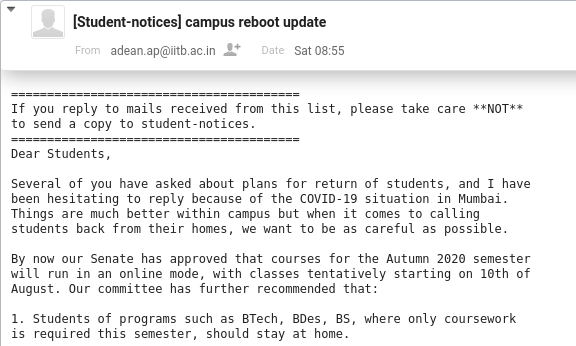
\includegraphics[width=0.6\linewidth]{Proof_of_online_semester.png} 
        \caption{Semester will be online, starting 10th August}
        \label{fig:img}
    \end{figure}

You can use \verb!floatrow! for inserting multiple images together.



















\end{document}